\chapter{TS upgrade roadmap}
This chapter will describe the changes that have been made to the interface
engine and how compatibility with legacy code is maintained.

\section{Interface upgrade}

\subsection{The legacy interface structure}
The legacy interface engine was programmed entirely in C++ and is developed against
using a set of C++ classes that the developer could combine into a tree structure.

Each class corresponds to an element in the Dojo library. These are things like
buttons, links, containers, \ldots .

Each class instance in this tree structure has its own string buffer.
This string buffer is initially filled with the default HTML and JavaScript code
to make the applicable Dojo element work.

Callbacks can be registered and attached to appropriate classes (e.g. an OnClick
event callback can be attached to a Button class), this allows the interface to
send data back to the server and will in turn allow the developer to change the
content of the string buffers.

After such a callback the current interface panel is reloaded and the interface
will contain any changes made in any of the string buffers.

\subsubsection{Page layout}
The main page contains a few div tags that are Dojo ContentPanes, these are used
as containers to display the panels, panel menus, and error messages if they come up.

The first ContentPane is `tsgui\_main\_`, it is placed directly under the body tag
and is not used client-side. Rather it is used in the legacy C++ code as a
container for the other panels.
In `tsgui\_main\_`, there is `tsgui\_dummyResult\_`, `tsgui\_treeBox\_`, and `tsgui\_content\_`.
These are used to display errors, the panel menus, and the interface panels,
respectively. This is also shown in figure \ref{fig:ts2_structure}.
\begin{figure}
  \centering
  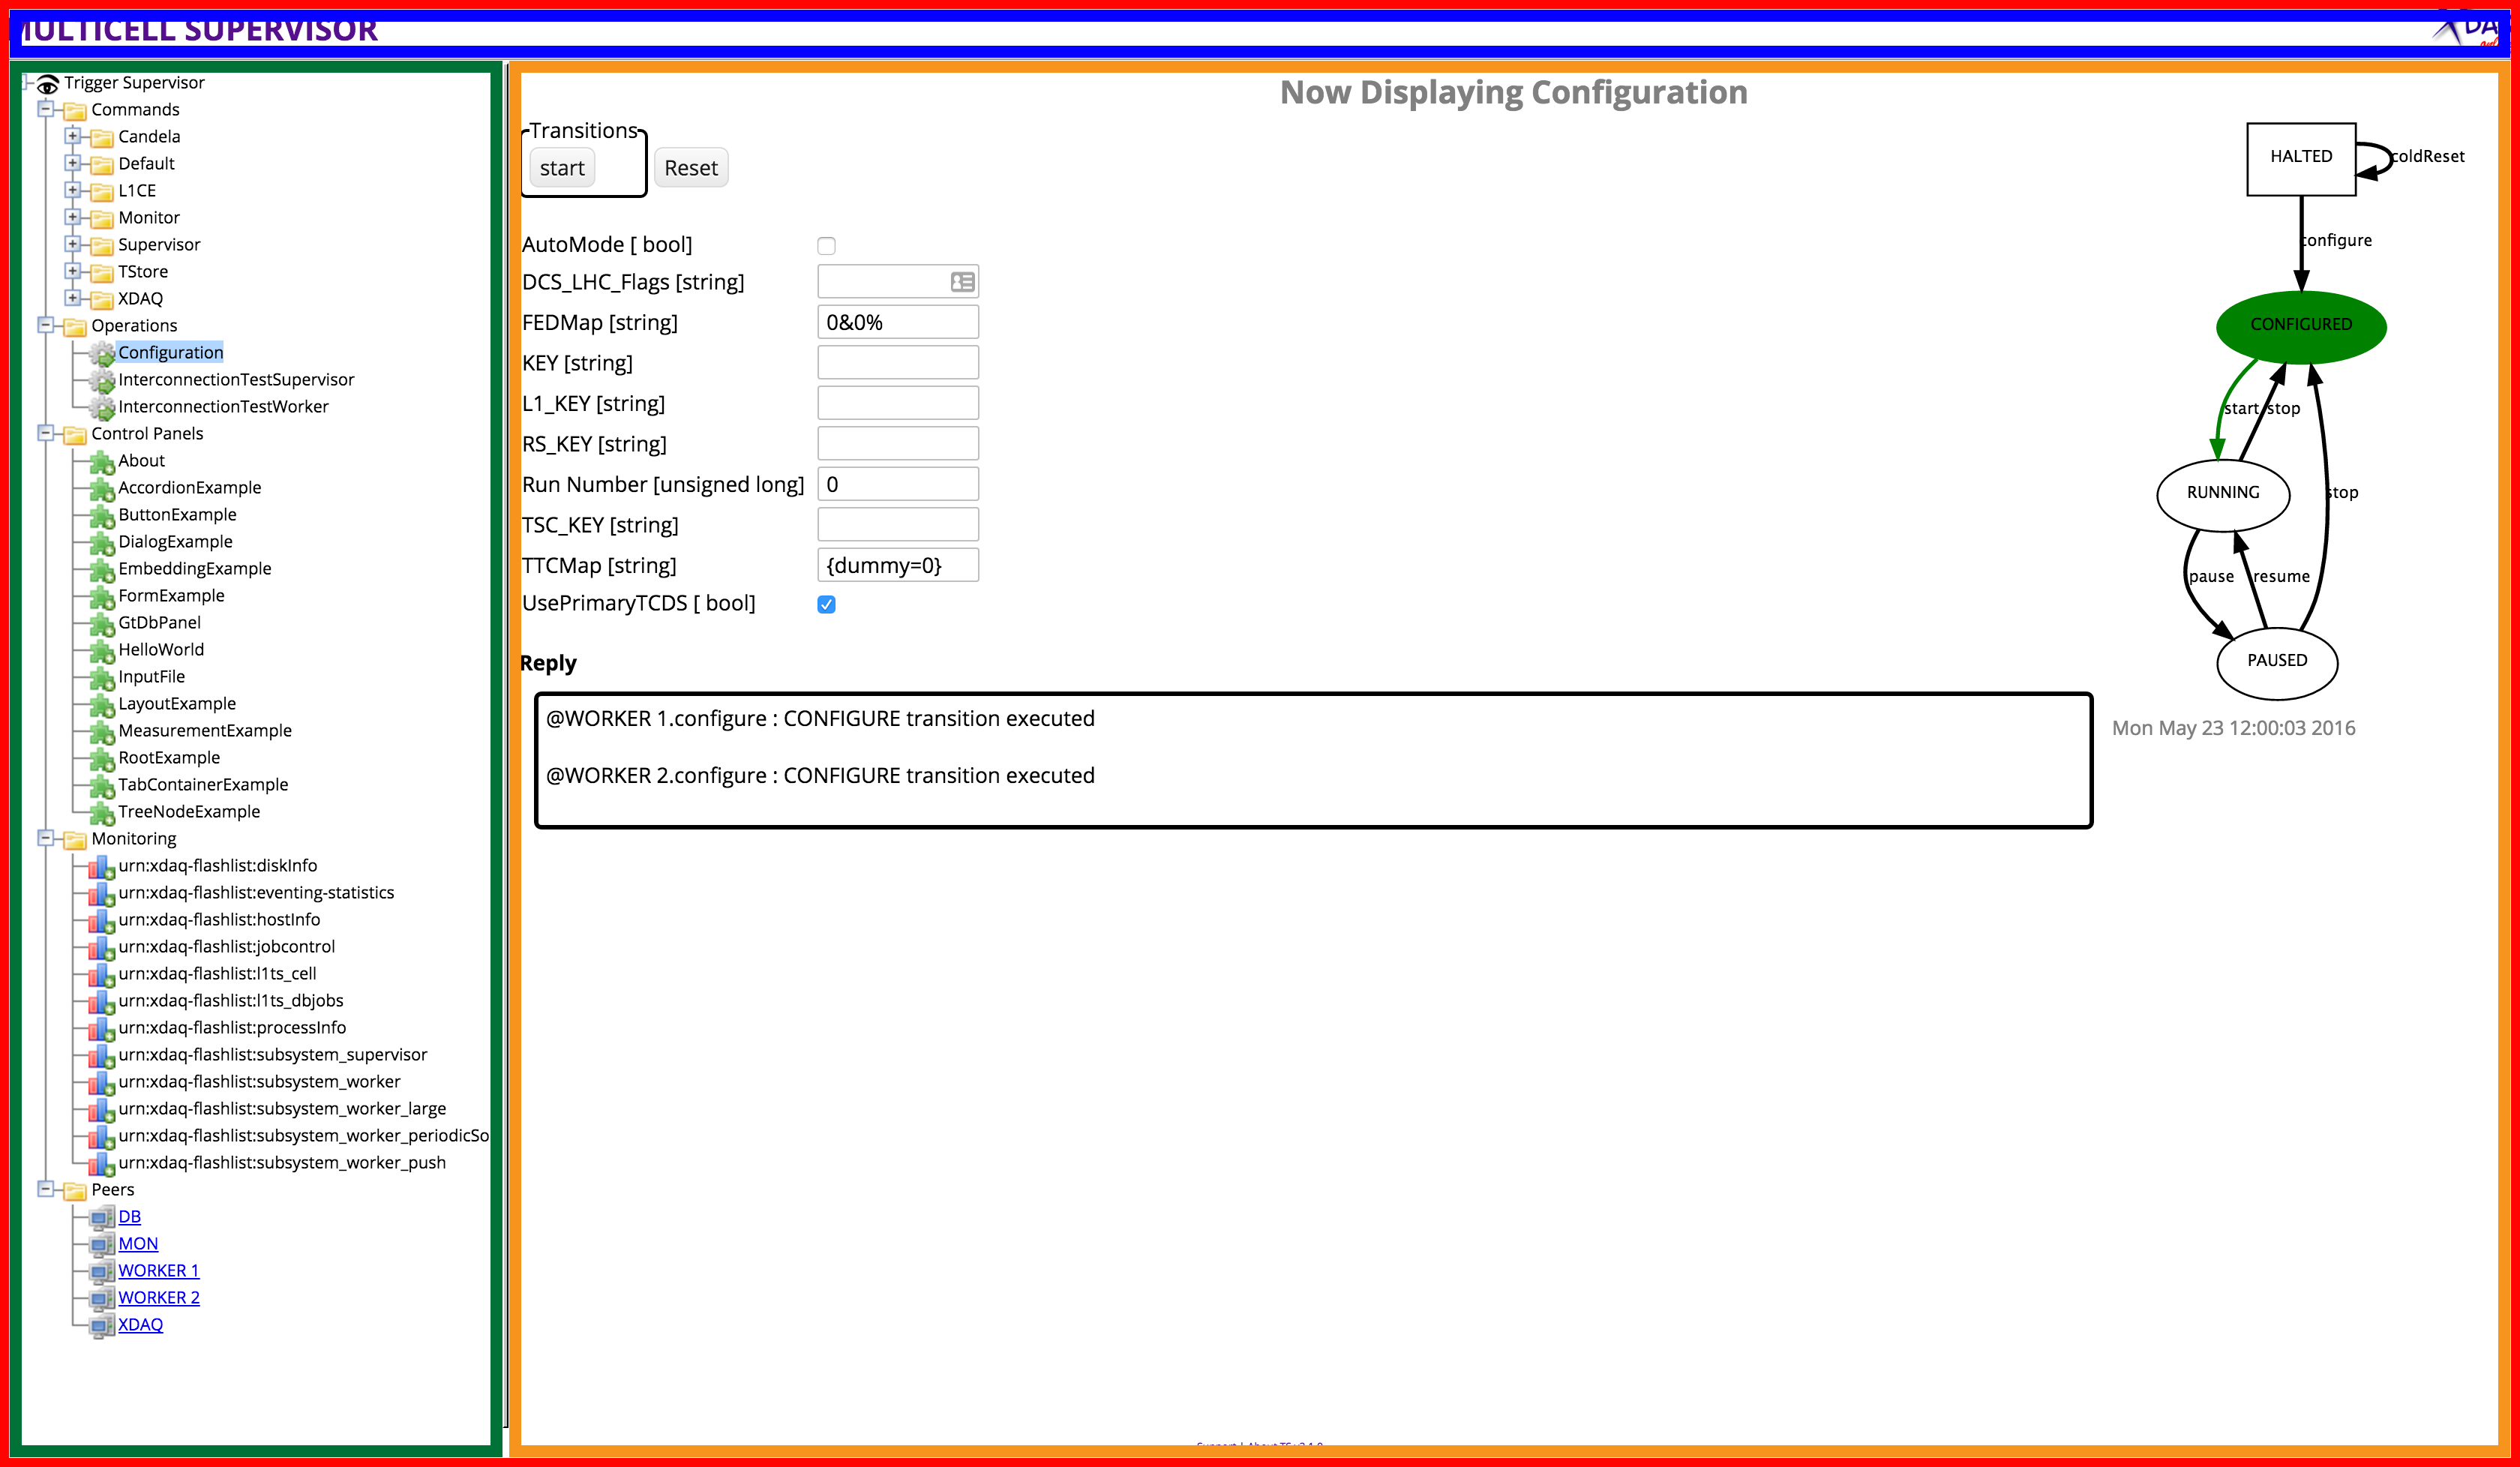
\includegraphics[width=\textwidth]{images/ts2_structure}
  \caption{Screenshot of TS v2.x with main components highlighted.}
  \label{fig:ts2_structure}
\end{figure}

In the new interface, only the `tsgui\_content\_` is kept. This is the Dojo container
where all the panels (legacy & Polymer) are displayed. The menu and top bar
are both handled client-side by a dedicated Polymer element. This is shown in
figure \ref{fig:ts3_structure}.
\begin{figure}
  \centering
  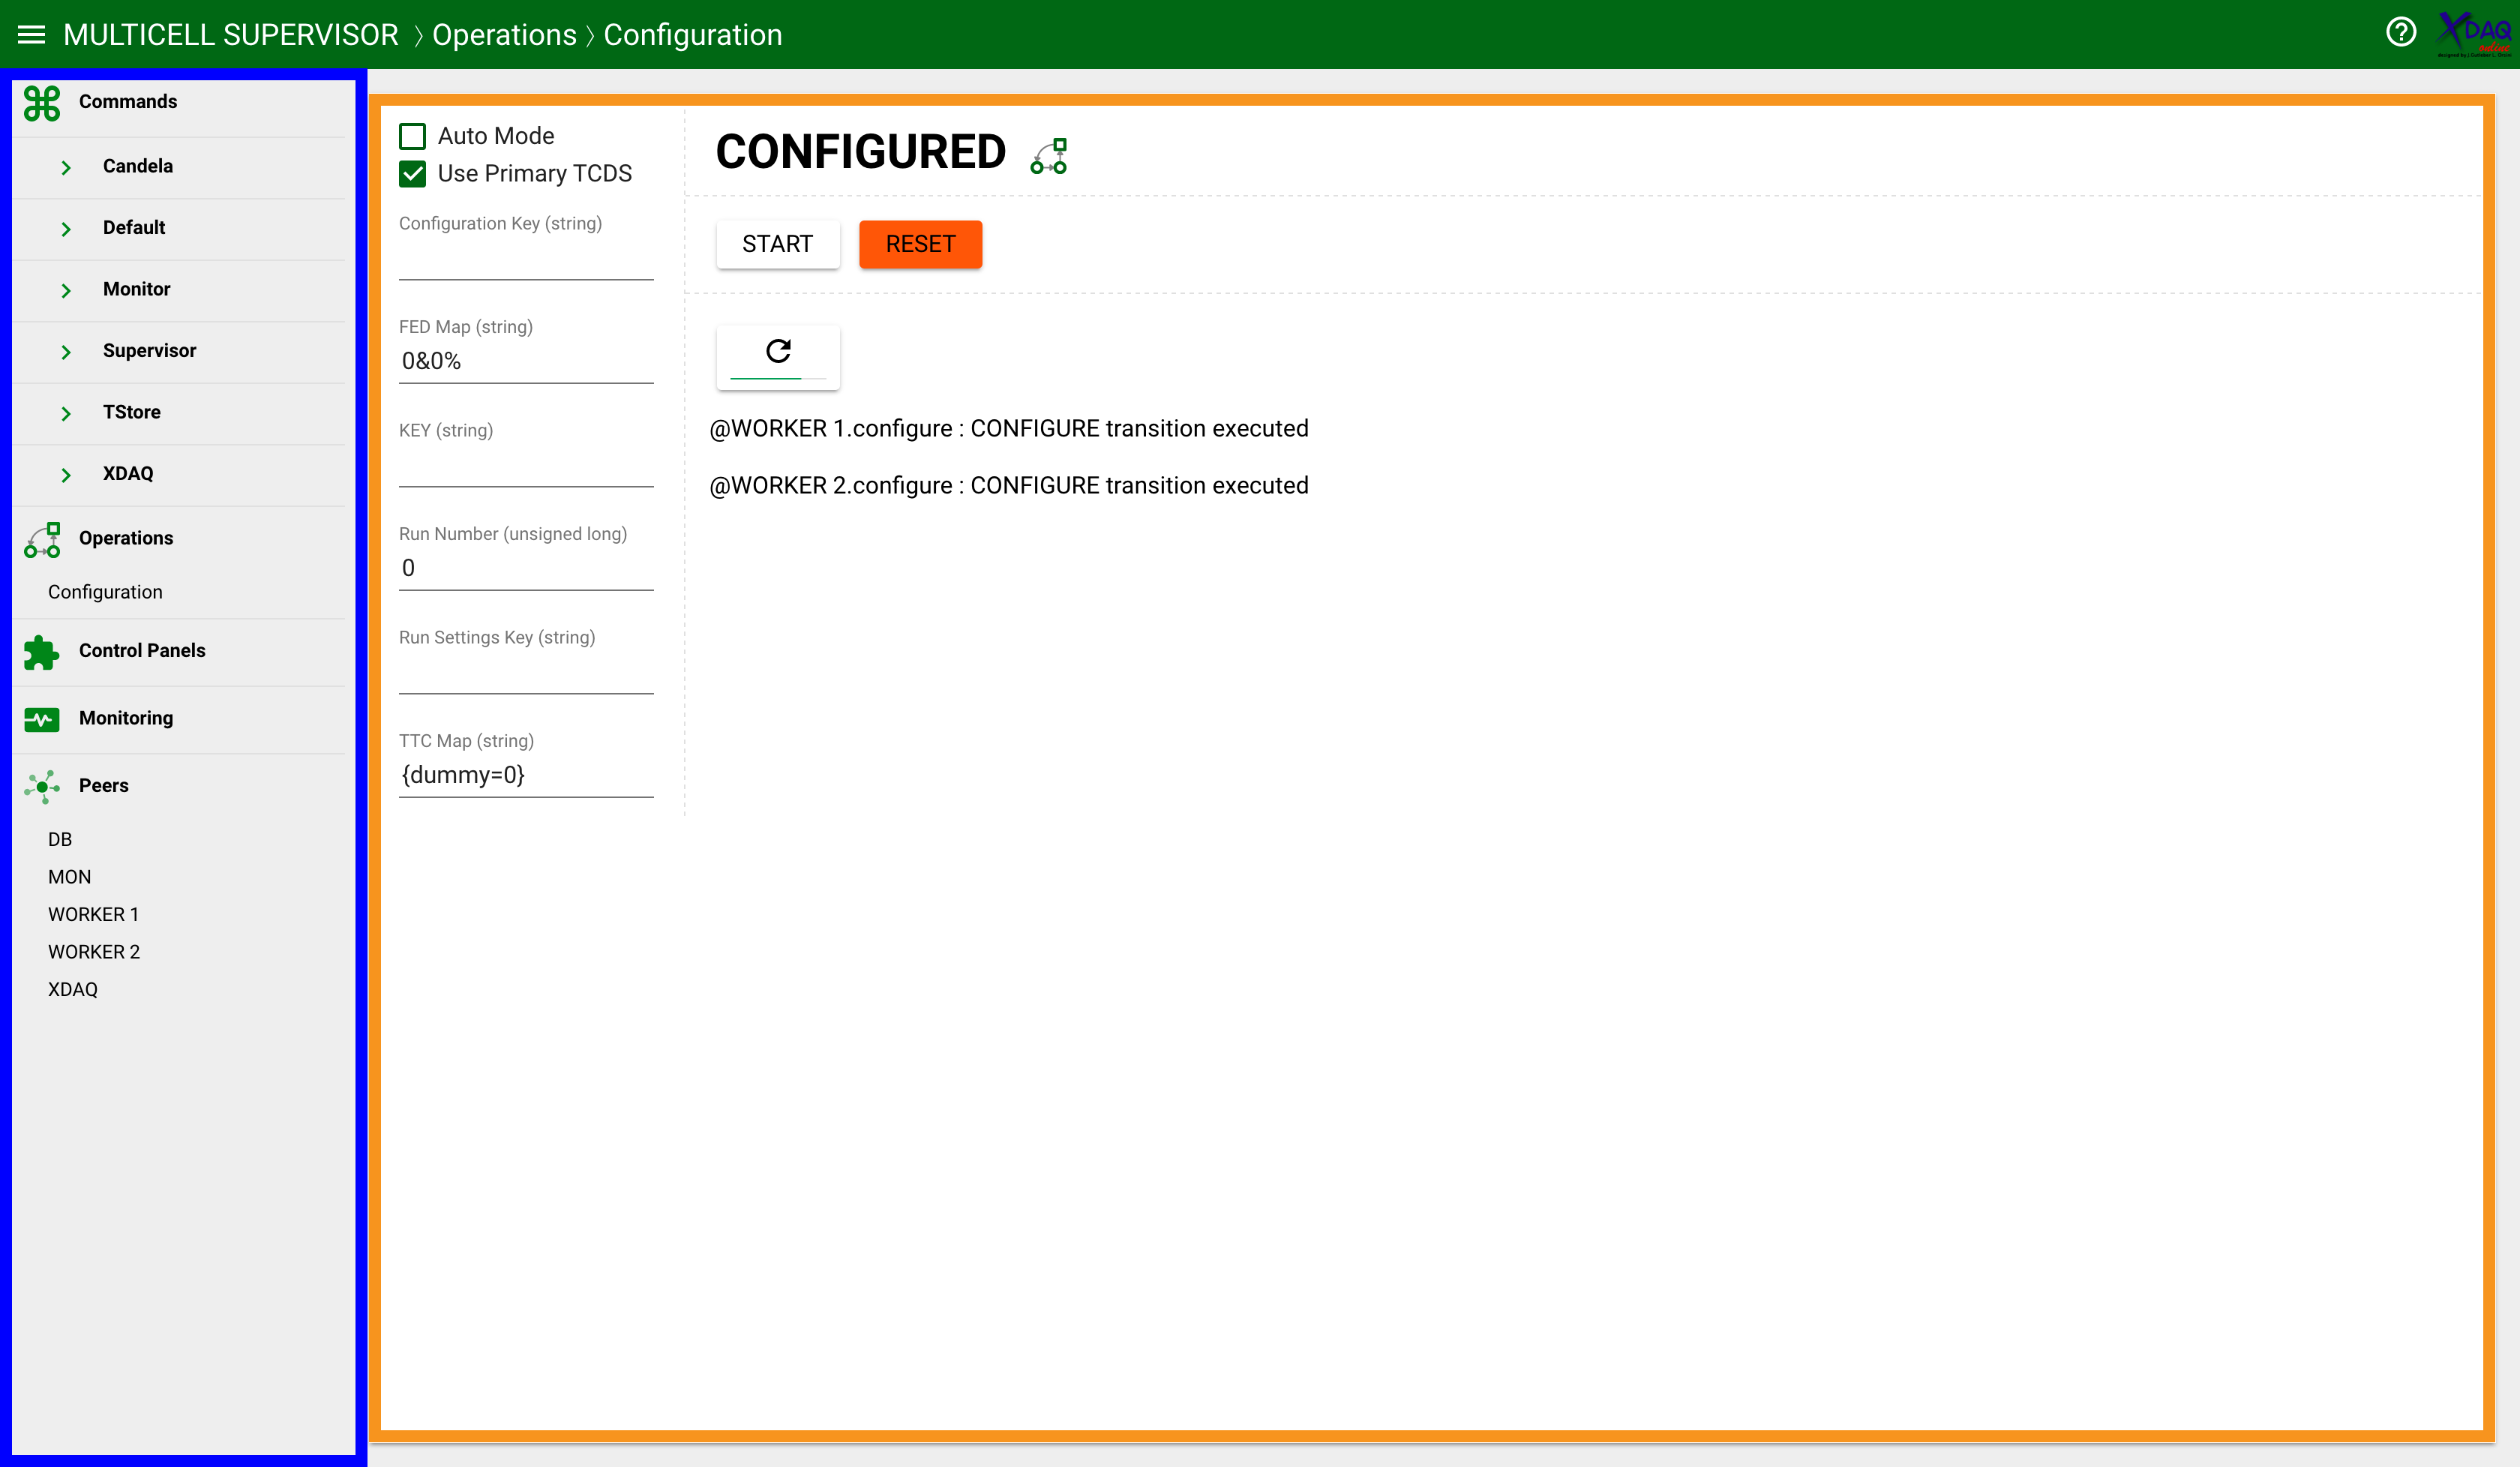
\includegraphics[width=\textwidth]{images/ts3_structure}
  \caption{Screenshot of TS v3.x with main components highlighted.}
  \label{fig:ts3_structure}
\end{figure}

\subsubsection{Session management}
The session is a 48-bit hexadecimal code, and is always encoded in the URL.
This way, if the user tries to interact with the server with an invalid session
token, the server can simply respond with a JavaScript payload redirecting them
to a URL containing a valid session ID.

The URL always looks like this
\begin{lstlisting}
http(s)://host:port/Default?_sesionid_=0x000000000000
\end{lstlisting}
Any state, e.g. the currently loaded panel, is kept server-side in the string
buffers.

\subsection{The new page structure}
The new interface will have the same general structure as the legacy interface,
though updated with the material design look and feel (see chapter \ref{Material Design}),
and some improvements (like a breadcrumb trail).

\subsection{Emulation of the legacy structure in the new page}
The new main page will keep the `tsgui\_content\_` Dojo ContentPane. This way
legacy Dojo panels can still be served, and since the ContentPane is just a plain
`div` tag when not using Dojo it won't inhibit any new code from functioning
properly.

\section{New session management}
The session ID will move out of the URL and will be moved into the response
headers of the server, this header will only be sent if a session change happened.

This approach has a few advantages:
\begin{itemize}
\item The session can now no longer be accidentally shared between users, since
it is no longer contained in the URL.
\item A session renewal does not require a full page reload. The panel will need
to be reset, as the user received a new session, but this will now be much faster
as it doesn't require a full reload.
\item In the old session system the user was navigated to the default page on a
session renewal, and did not preserve the user's navigation through the cell
interface like the new session system does.
In the new system the interface detects the presence of a new session id in any
response of the server, and executes appropriate code to handle a session renewal.
\end{itemize}

\subsection{Material Design}
\label{Material Design}
Material Design (previously called Quantum Paper) is a design language developed
by Google\cite{materialdesign_launch}, released in 2014. It aims to return to the design principles used
in printing, and extend it with things that are normally not possible in real
printing (e.g. motion, responsive layouts, \ldots).

At the center of material design is paper, every component of the design spec
treats a user interface element (e.g. containers, buttons, dropdowns, \ldots) as
a it was being cut out and pasted together with paper.
The reason for this is that it is easier for a user to think with physical objects,

Google uses it to bring back consistency throughout its product line and across
all types of devices. Material design is deployed on watches, phones, tablets,
laptops, and televisions.
Android Marshmallow (v6.x) has fully migrated to material design, and the vast
majority of apps in the Google Play store have adopted it.

The full Material Design spec can be found on the Google design webpage\cite{materialdesign}.

\section{Handling large input}
The legacy (i.e. Dojo) panels sent data back to the server using URL encoding
(more info in chapter \ref{Large input problem}).

The legacy panels can't be adjusted without risking unforeseen consequences.
The new (i.e. Polymer) panels however will all send data back to the server
properly, using HTTP POST requests that contain any parameters in the POST body.

This is the way the HTTP specification designed to send data back to a server,
and thus it solves the problems encountered with sending data with the
legacy code. With the new approach it is now theoretically possible to send 
multi-gigabyte sized data.

\section{Additions to the page builder classes}
The C++ classes in the legacy system each represent an HTML element.
This is manageable because in the set of elements in the legacy system is fixed.
% In the legacy system the set of elements is fixed.
Since in the new system every interface developer will now have the possibility to extend the set of
elements it would make sense to make a more abstract class to handle these new
set of elements.

The ajax::PolymerElement class was added and is used like follows:
\fvset{frame=single}
\begin{pyglist}[language=cpp,numbers=left,numbersep=5pt,fontsize=\small]
ajax::PolymerElement* myElement = new ajax::PolymerElement("my-element");
myElement->set("some-property", "someValue");
add(myElement);
\end{pyglist}
\fvset{frame=none}

Furthermore, the PlainHtml class has been extended with some shorthand functions
to make it easier to use. This because it is a frequently used class.
instead of doing:
\fvset{frame=single}
\begin{pyglist}[language=cpp,numbers=left,numbersep=5pt,fontsize=\small]
ajax::PlainHtml* br53 = new ajax::PlainHtml?();
br53->getStream() << " <p>some html code<p>";
add(br53);
\end{pyglist}
\fvset{frame=none}
it is now possible to do this:
\fvset{frame=single}
\begin{pyglist}[language=cpp,numbers=left,numbersep=5pt,fontsize=\small]
add(new ajax::PlainHtml(" <p>some html code<p>"));
\end{pyglist}
\fvset{frame=none}
This greatly enhances readability of pages containing a lot of arbitrary html code like `<br>`

The AjaXell code has also been modified to support HTML5 features like boolean
attributes (i.e. attributes with no value).

\section{Upgraded event system}
In the legacy codebase, events are attached to C++ classes declared in a panel.
\fvset{frame=single}
\begin{pyglist}[language=cpp,numbers=left,numbersep=5pt,fontsize=\small]
ajax::Button* button = new ajax::Button();
button->setId("subsystem_btnpanel_button_");
button->setCaption("click me!");
this->setEvent(button,ajax::Eventable::OnClick,result_,this,&ButtonExample::onClick);
add(button);
\end{pyglist}
\fvset{frame=none}

However, this system has been extended to allow an event to be attached to the
panel itself, rather than a class instance defined in the panel code.
\fvset{frame=single}
\begin{pyglist}[language=cpp,numbers=left,numbersep=5pt,fontsize=\small]
setEvent("submit", ajax::Eventable::OnClick, this, &FormExample::submit);
add(new ajax::PolymerElement("form-example"));
\end{pyglist}
\fvset{frame=none}

This is necessary because the server will no longer render every element in the
interface. An element (e.g. a button) can be rendered client-side, so

\section{New JSON library}
The primary job of the server-side code will no longer be interface generation,
but data generation.

In the legacy codebase there has been no easy way to generate XML or
JSON data. The only viable way to construct these were to construct them manually
or to use BOOST Property Trees, which require extensive amounts of code.

The TS will incorporate the JsonCpp library, a lightweight C++ library that
makes the generation and parson of JSON very easy.

More information about this can be found in chapter \ref{JsonCpp}.

\section{Memory-leak problem}
\label{Memory-leak problem}
An interface panel can be used for extensive amounts of time, this time can be
expressed in days. Therefore any memory leaks are unacceptable.

Unfortunately it is rather easy to create memory leaks in JavaScript.
JavaScript uses a Reference-counting garbage collection system\cite{IBM_MemoryLeaks}.
Such a garbage collector cannot recognize circular references, and JavaScript
closures add another memory leak pattern to watch out for.

\subsection{Memory-leak patterns}
\subsubsection{Circular references}
A circular reference is formed when two or more objects reference each other in
such a way a closed circle can be drawn.
\begin{figure}[H]
  \centering
  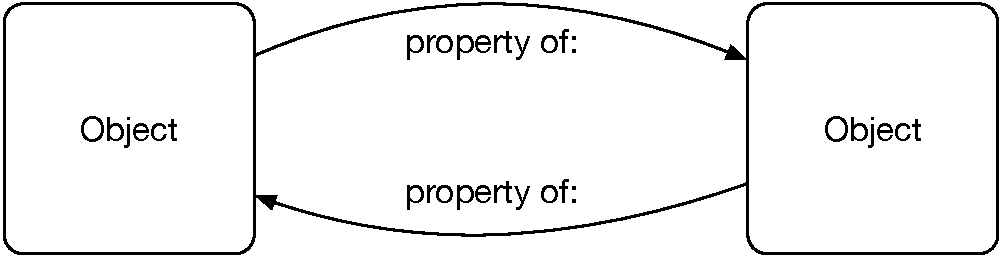
\includegraphics[width=.5\textwidth]{images/circular_reference}
  \caption{A circular reference}
  \label{fig:circular_reference}
\end{figure}

In a reference counting garbage collector like JavaScript these kind of
structures present problems because there is no way the reference count of any
of the object in a circular reference can reach zero, and thus will never be
garbage collected.

The following code will create a circular reference.
\fvset{frame=single}
\begin{pyglist}[language=html,numbers=left,numbersep=5pt,fontsize=\small]
<html>
  <body>
    <div>an HTML element</div>
    <script>
      var div=document.querySelector("div");
      div.someproperty = div;
    </script>
  </body>
</html>
\end{pyglist}
\fvset{frame=none}

This piece of code will however not appear very often. There is not a real use
case where this would appear, and the memory leak is rather obvious.

\subsubsection{JavaScript closures}
A feature of JavaScript is that functions can contain other functions. The inner
function will inherit variables from the parent function.

This inheritance of variables by inner functions is called closure.
This is a code example demonstrating closure:
\fvset{frame=single}
\begin{pyglist}[language=javascript,numbers=left,numbersep=5pt,fontsize=\small]
window.onload = function() {
  var test = 5;
  function innerfn() {
    // will display 5
    alert(test);
  }
  innerfn();
}
\end{pyglist}
\fvset{frame=none}

Closures are the cause of most memory leaks in JavaScript.
Consider the following use case:

An element is created, and a callback is attached to it to react to the click event.
\fvset{frame=single}
\begin{pyglist}[language=javascript,numbers=left,numbersep=5pt,fontsize=\small]
var newelement = document.createElement('p');
newelement.textContent = 'click me';
newelement.onclick = function() {
  alert("you clicked me");
}
document.body.appendChild(newelement);
\end{pyglist}
\fvset{frame=none}
This simple code example contains a memory leak. the function attached to the
onclick event inherits the `newelement` variable, and thus has created a
circular reference.

\subsubsection{Avoiding memory leaks}
Some simple patterns exist to avoid circular references.

Firstly, in a parent function one can set one of the variables causing a
circular reference to null, thereby breaking the circle.
\fvset{frame=single}
\begin{pyglist}[language=javascript,numbers=left,numbersep=5pt,fontsize=\small]
var newelement = document.createElement('p');
newelement.textContent = 'click me';
newelement.onclick = function() {
  alert("you clicked me");
}
document.body.appendChild(newelement);
newelement = null;
\end{pyglist}
\fvset{frame=none}

Another approach is to insert another closure
\fvset{frame=single}
\begin{pyglist}[language=javascript,numbers=left,numbersep=5pt,fontsize=\small]
var inner2 = function() {
  alert("you clicked me");
}
(function inner() {
  var newelement = document.createElement('p');
  newelement.textContent = 'click me';
  newelement.onclick = inner2;
  document.body.appendChild(newelement);
})();
\end{pyglist}
\fvset{frame=none}

Lastly, one can avoid closure altogether.
\fvset{frame=single}
\begin{pyglist}[language=javascript,numbers=left,numbersep=5pt,fontsize=\small]
function callbackfn = function() {
  alert("you clicked me");
}
var function makeElement = function() {
  var newelement = document.createElement('p');
  newelement.textContent = 'click me';
  newelement.onclick = callbackfn;
  document.body.appendChild(newelement);
}
makeElement();
\end{pyglist}
\fvset{frame=none}

\subsection{Memory leaks in Dojo}
\label{Memory leaks in Dojo}
Unfortunately, Dojo 0.4 or the implementation used here seems to contain a lot
of circular references. Memory usage goes up linearly with the amount of panels
used in a browser session.

To test this, a panel will be reloaded (by clicking in the menu) every second.
This will be done for a period of ten seconds, following a 10 second idle period
to allow for any garbage collection to trigger.
This cycle will be executed for sixty seconds, and will be followed by a final
sixty second idle period to make sure any garbage collection has occurred.

The results for this test for TS v2.1.0 is displayed in figure \ref{fig:ts2_memory}.
\begin{figure}
  \centering
  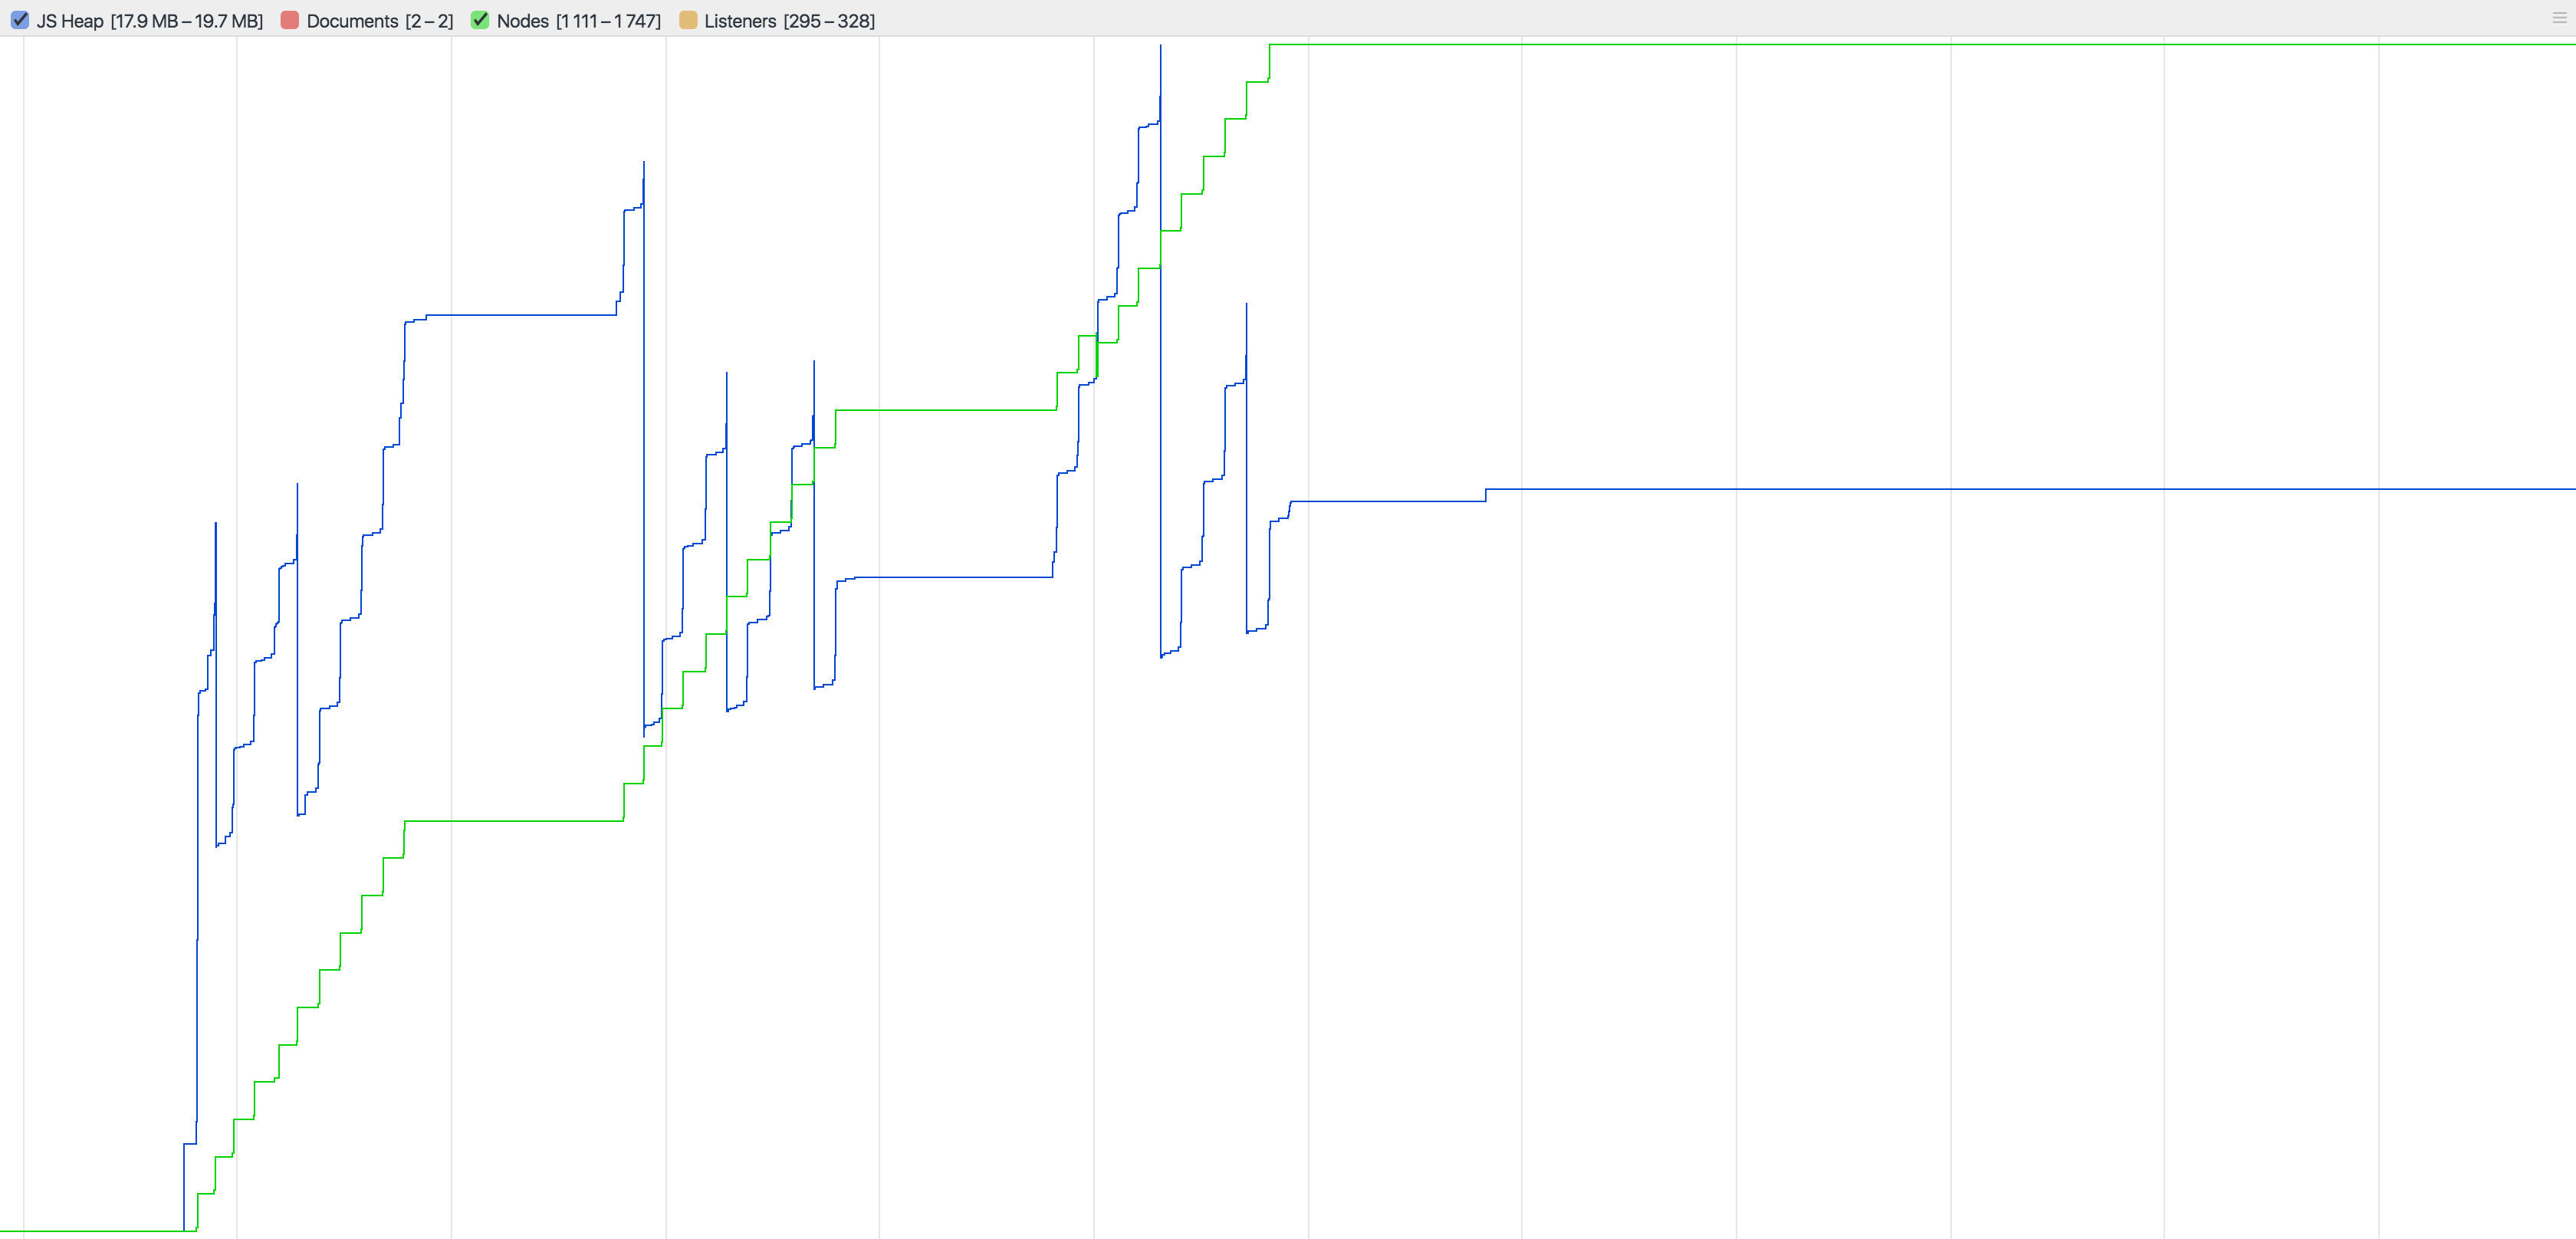
\includegraphics[width=\textwidth]{images/dinosaurs-are-great-120s-run}
  \caption{TS 2.x interface memory usage test}
  \label{fig:ts2_memory}
\end{figure}
Notice that the amount of nodes does not go down. This is because of the circular
references described earlier. The garbage collector will never remove these nodes
from memory, because the reference count of these nodes will never reach zero.

As a result, the memory consumption will grow arbitrarily as panels are used.

In the TS 2.x interface this was not noticed because of the very frequent full
page reloads.
However, with the new graceful session renewal that does not require a page
reload, these memory leaks in dojo panels will pile up until the user manually
refreshes the browser.

Figure \ref{fig:ts3_legacy_memory} shows the result of the same test in the
TS 3.x interface, with the same legacy panel used to test the TS 2.x.
\begin{figure}
  \centering
  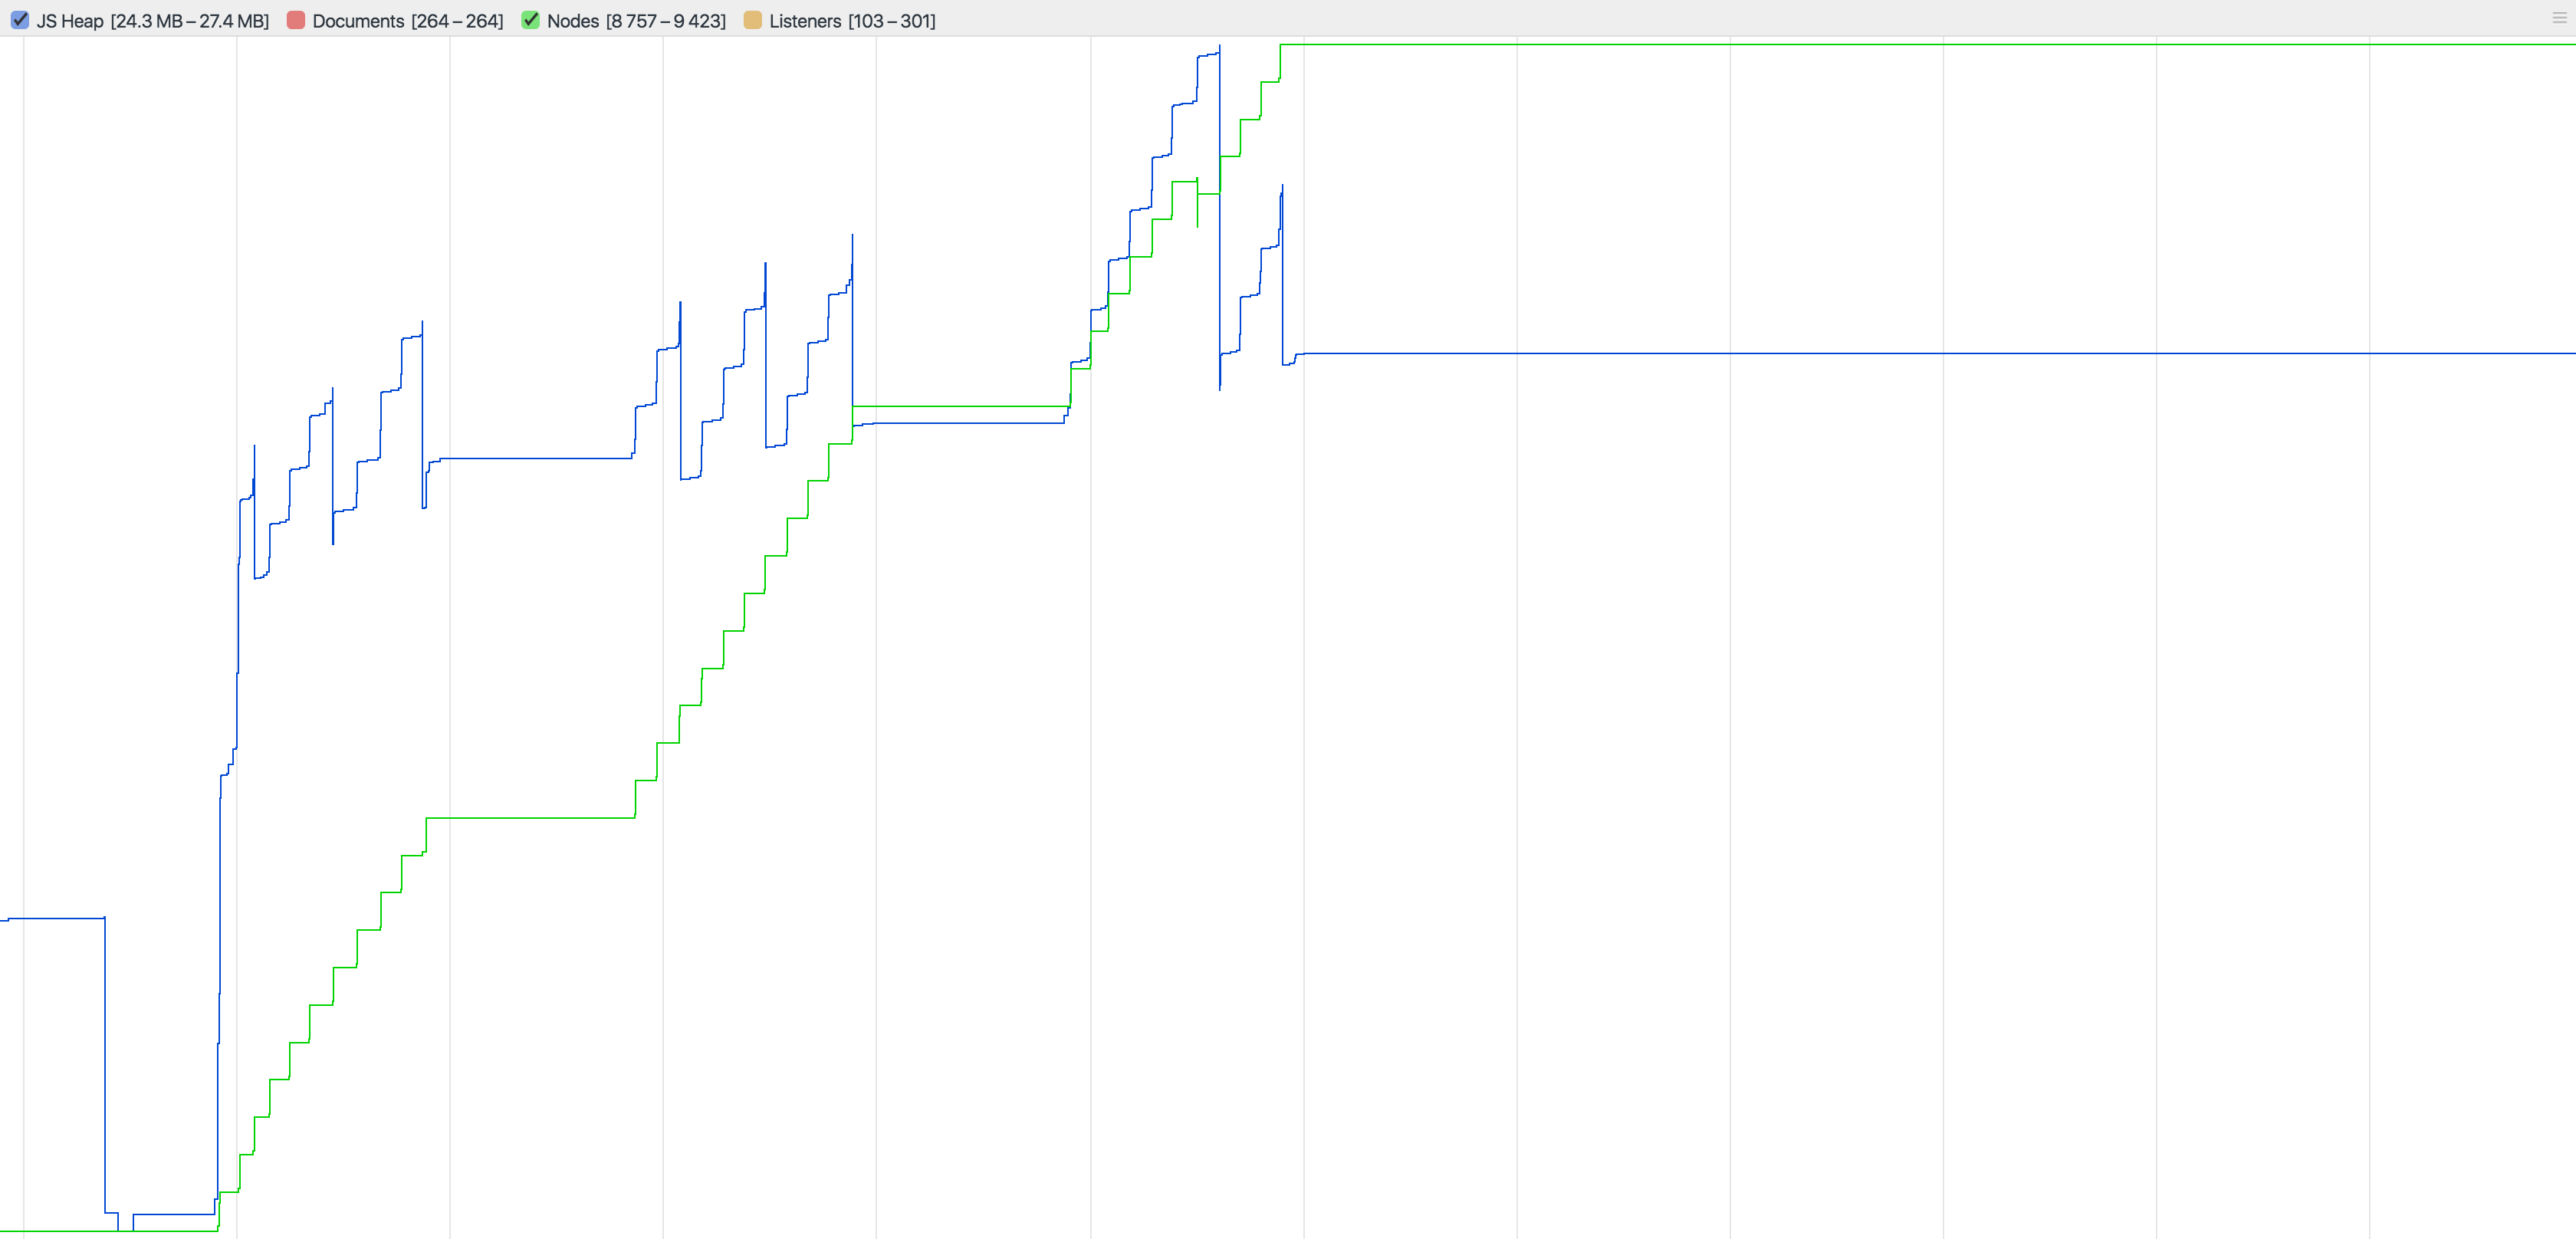
\includegraphics[width=\textwidth]{images/kill-all-roommates-120s-run}
  \caption{TS 3.x interface memory usage test with a legacy panel}
  \label{fig:ts3_legacy_memory}
\end{figure}

Despite the rewritten main interface, the memory leak still occurs with legacy
panels. This is because the cause of the memory leak resides inside the Dojo
library itself.

A solution to this problem is not easily apparent. It would require changes to
the legacy codebase, which is always a risky thing to do.
It is decided that for this reason, any legacy panel that features automatic
refreshes (e.g. the operations panel) has a high priority to be replaced with a
polymer alternative.

\subsection{Memory leaks in Polymer}
\label{Memory leaks in Polymer}

The same test is done again in the TS 3.x interface, but with the panel being
upgraded to a Polymer equivalent. The results are shown in figure \ref{fig:ts3_memory}.

Note that this time, the garbage collector is able to remove unused DOM nodes
from memory, followed by the memory usage returning to its original value
immediately after the test.

\begin{figure}
  \centering
  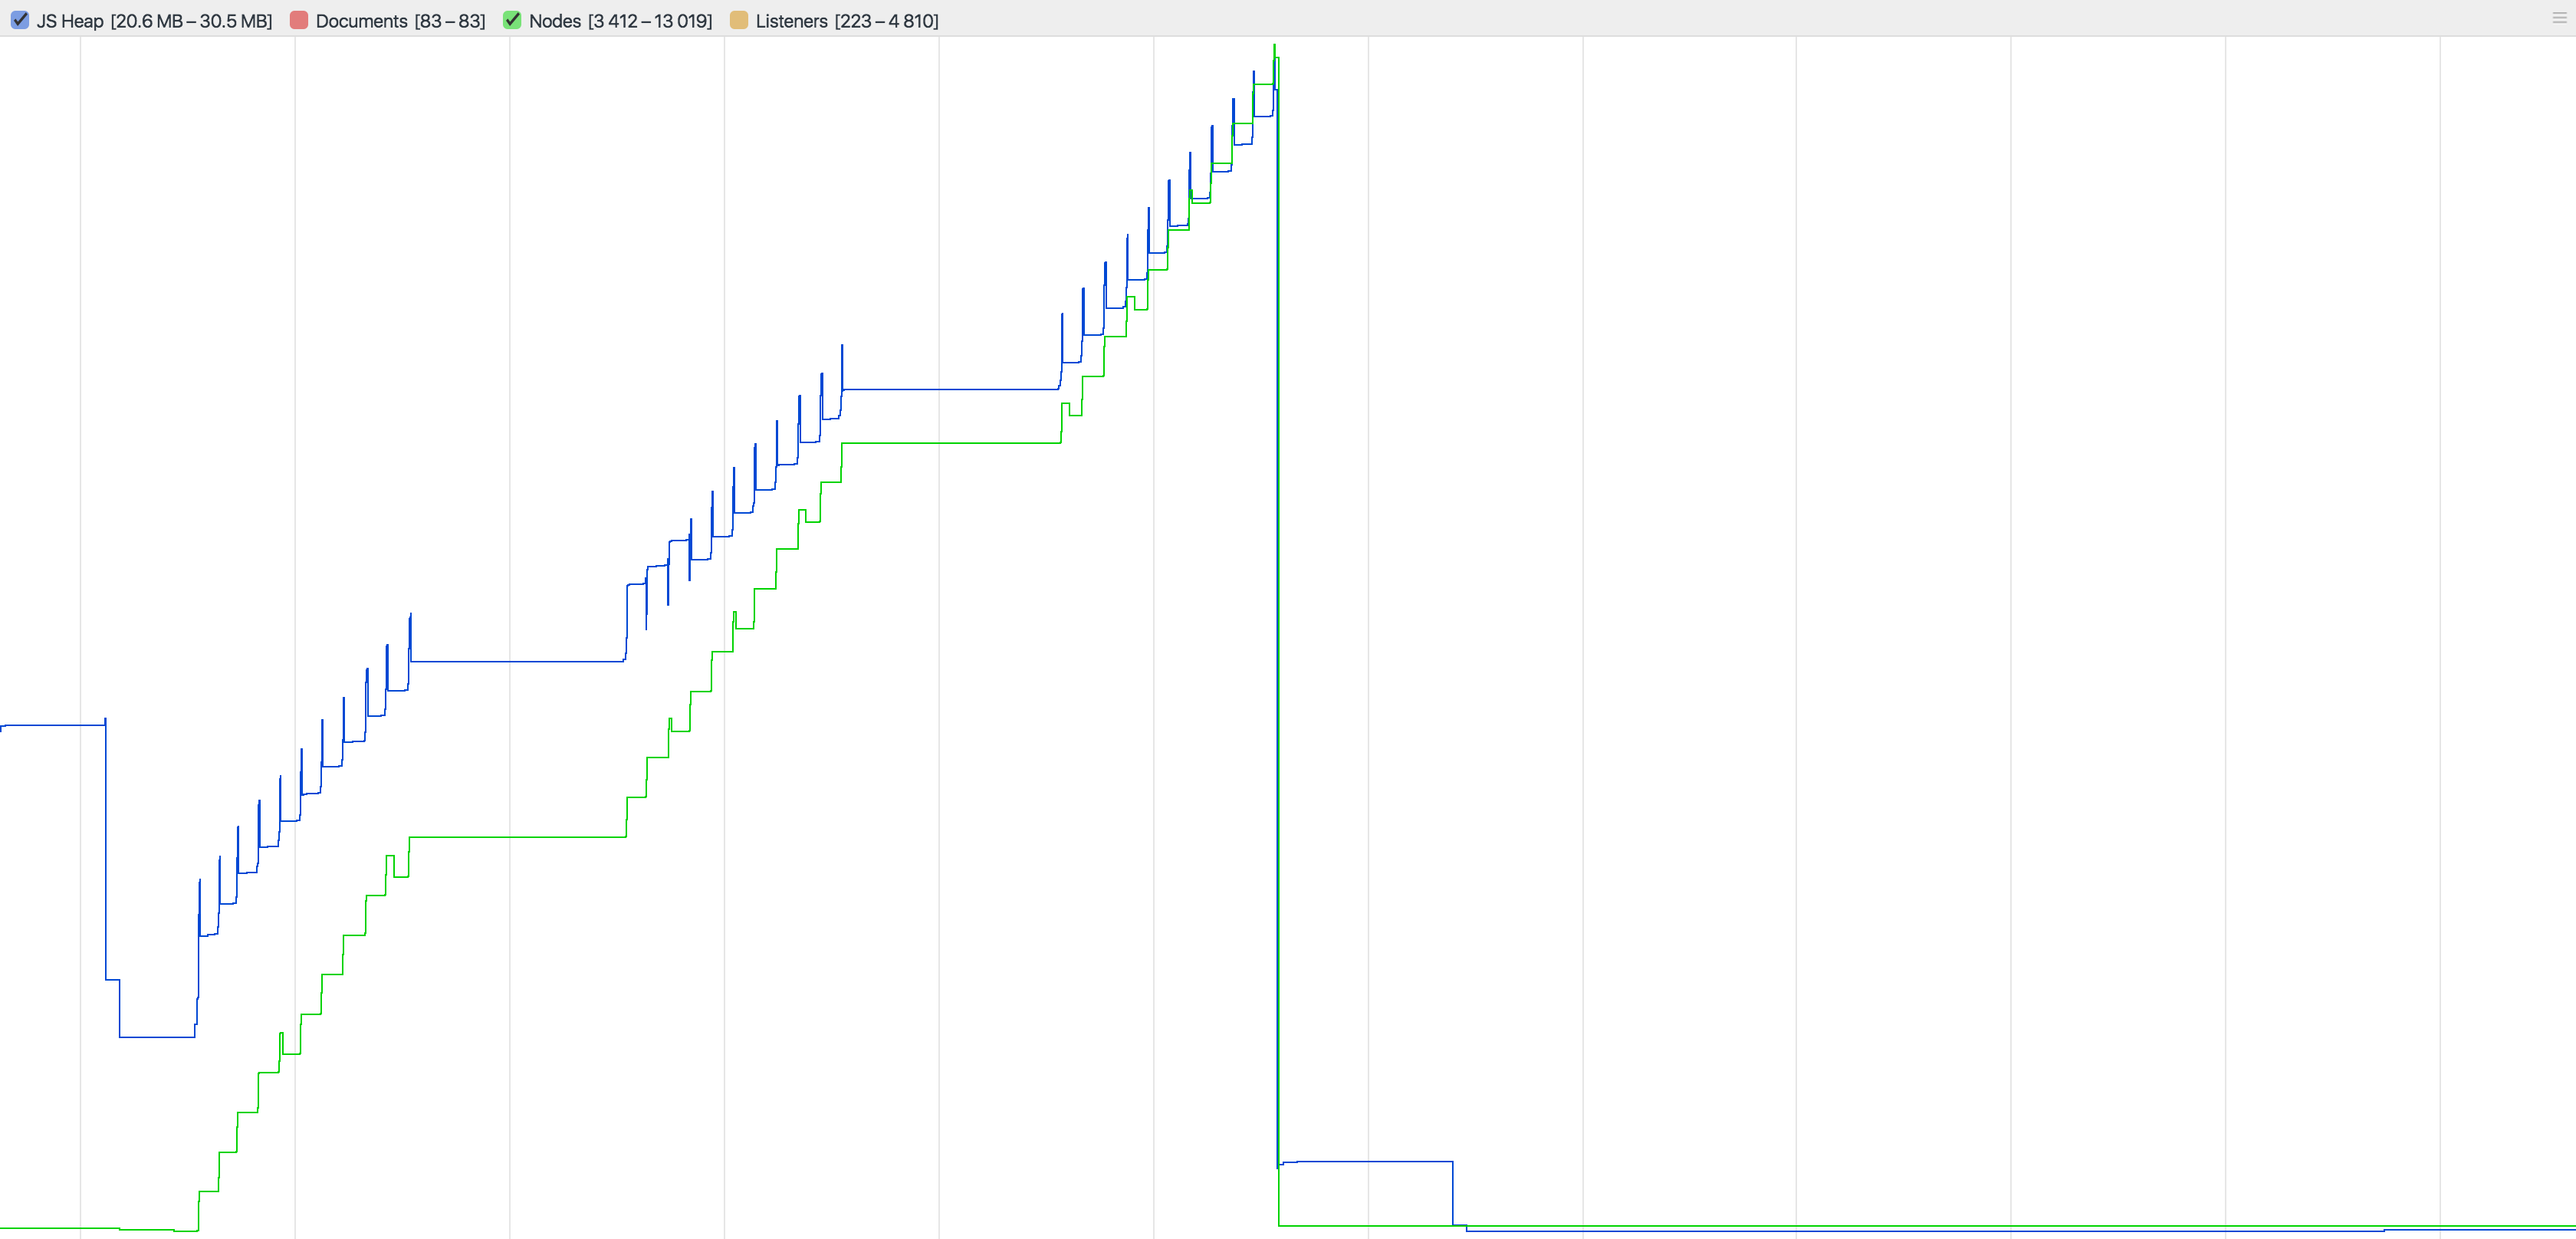
\includegraphics[width=\textwidth]{images/kill-all-humans-120s-run}
  \caption{TS 3.x interface memory usage test with a Polymer panel}
  \label{fig:ts3_memory}
\end{figure}
